\newSec[Flight]{Analyse realer Flugdaten}{1}

In diesem Kapitel werden die Daten eines Testflugs mit der \Ar\ analysiert.






\newSec[FlightProcess]{Verlauf}{2}
Dieses Kapitel zeigt die verschiedenen Daten des Flugs, um diese in der nachfolgenden Analyse einordnen zu können.



\begin{figure}[ht!]
\vspace{0.25cm}
\begin{center}
\fbox{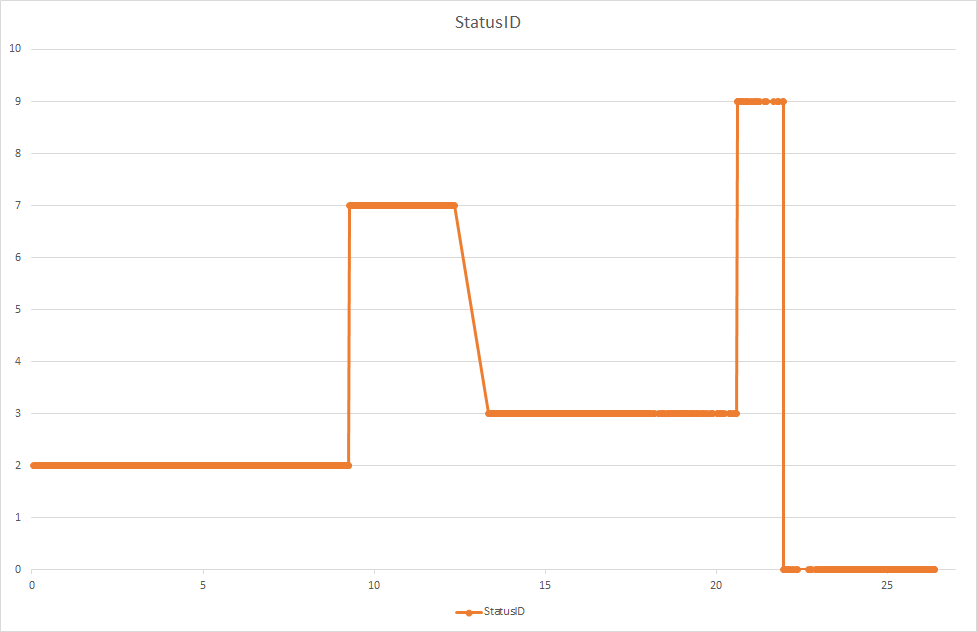
\includegraphics[width=15cm]{Pictures/Flight StatusID.png}}
\caption{Testflug: StatusID}
\label{fig:FlightStatus}
\end{center}

\vspace{0.25cm}
Der Testflug wird mit der Aufforderung der Status-Änderung bei etwa 9.3 s initialisiert. Davor befindet sich der \Quad\ ruhend auf einer ebenenen Oberfläche.
Die hier eingenommene StatusID = 7 entspricht \glq Goto Fix Point\grq, wobei hier vermutlich eine Höhe von 0.4 m angenommen werden soll. Zwischen etwa 12.3 s und 13.3 s wird keine Nachricht zum aktualisieren der Daten gesendet. Anschließend wechselt der Status zu \grq Flying\glq.
Die Status-Änderung bei etwa 20.6 s entspricht einer Notlandung aufgrund niedriger Batterieladung.
\end{figure}


\begin{figure}[ht!]
\vspace{0.25cm}
\begin{center}
\fbox{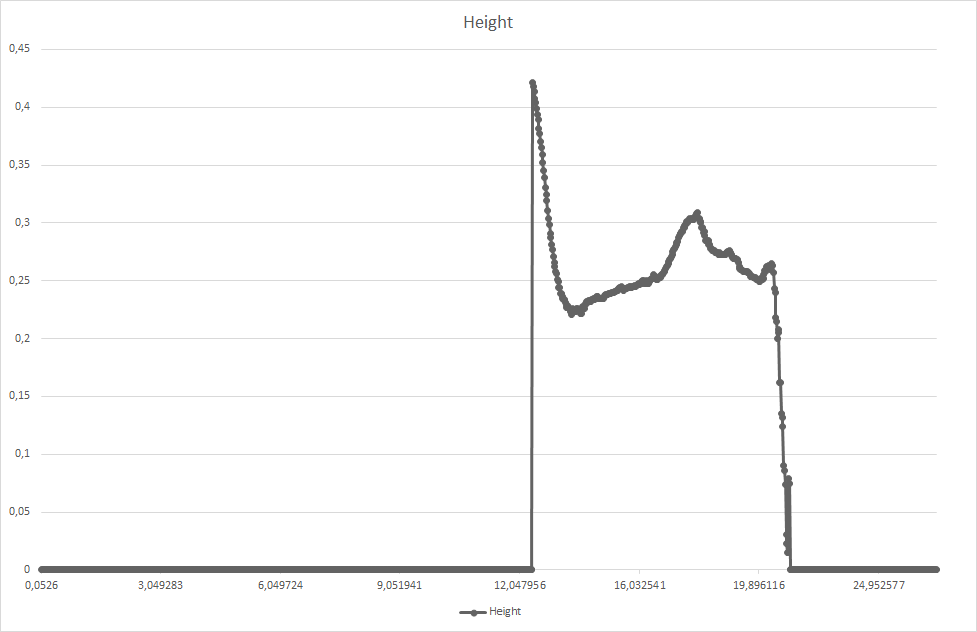
\includegraphics[width=15cm]{Pictures/Flight Height.png}}
\caption{Testflug: Höhenverlauf}
\label{fig:FlightHeight}
\end{center}

\vspace{0.25cm}
Äquivalent zu \refImg{fig:FlightStatus} zeigt sich der Verlauf des Höhenprofils des Fluges. Die Daten wurden von der Ultraschall-Messung abgegriffen. Eine Transformation der Einheiten in [$m$] wurde vorgenommen.
\end{figure}


\begin{figure}[ht!]
\vspace{0.25cm}
\begin{center}
\fbox{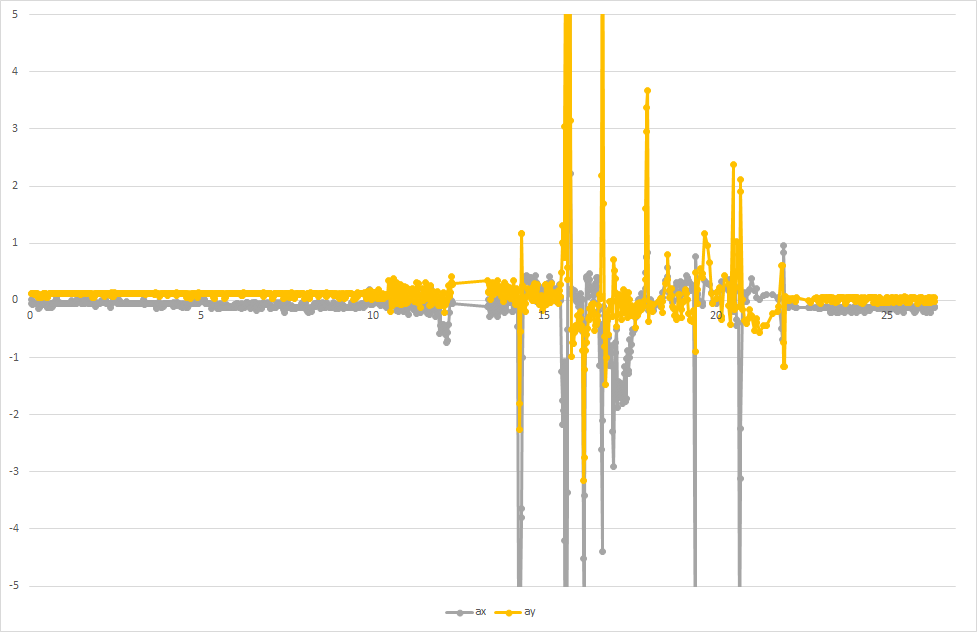
\includegraphics[width=15cm]{Pictures/Flight ax ay.png}}
\caption{Testflug: Beschleunigung zx- und y-Achse}
\label{fig:Flightaxay}
\end{center}

\vspace{0.25cm}
Zu sehen sind die gemessenen Beschleunigungswerte der horizontalen Achsen. Ausreißer wurden in dieser Grafik ignoriert, um einen detallierteren Verlauf kleinerer Werte ersichtlich zu machen. An dieser Stelle soll auf die Nullpunkt-Abweichung der Beschleunigungsdaten hingewiesen werden.
Die Ausreißer können teilweise auf Berührungen des \Quad[s] mit einem Hindernis (Wand) zurückgeführt werden. 
\end{figure}



\begin{figure}[ht!]
\vspace{0.25cm}
\begin{center}
\fbox{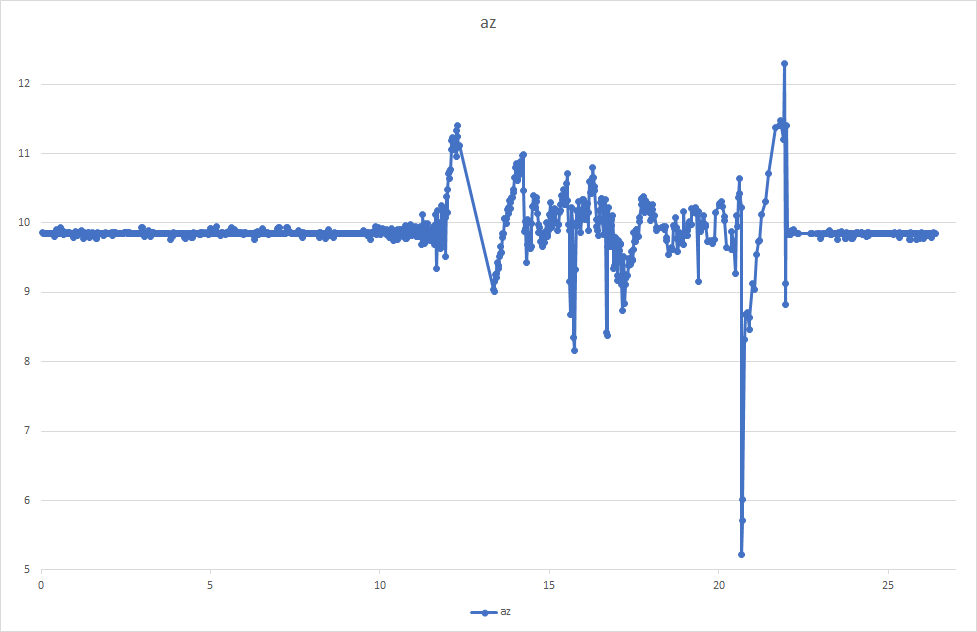
\includegraphics[width=15cm]{Pictures/Flight az.png}}
\caption{Testflug: Beschleunigung z-Achse}
\label{fig:Flightaz}
\end{center}

\vspace{0.25cm}
Der Anstieg bei etwa 12 s entspricht dem Abheben des \Quad[s].\\
Der Ausreißer nach unten bei etwa 21 s entspricht der Initialisierung der Landung, gefolgt von einem Ausreißer nach oben bei etwa 22 s, welcher das Auftreffen des \Quad[s] auf dem Untergrund anzeigt. Hier ist von korrekt gemessenen Werten auszugehen.
\end{figure}



\missing[Analyse mit Daten der parrot Drohne]









\FloatBarrier
\newSec[FlightAnalysis]{Analyse}{2}


\newSec[FlightAnalysisLeak]{Lecks der Datenübertragung}{3}

\missing[Beim Start etwa 1s, etwas später nochmal ein bisschen Probleme...]





\newSec[FlightAnalysisOffset]{Offset der Beschleunigungswerte}{3}

Wie \refImg{fig:Flightaxay} entnommen werden kann, sind die Werte für die Bescleunigungen entlang der x- und y-Achsen nicht auf den Wert 0 kalibriert. Eine Kalibrierung des \Quad[s] wird unmittelbar vor dem Start gesendet und kann auch unabhängig durch eine User-Eingabe ausgelöst werden.

Die Gravitation ist in \refImg{fig:Flightaz} ablesbar.

Entsprechend \refCap{ControlPosAccelOffset} sind diese Abweichungen zu korrigieren.
Als Ansatz kann hier eine Mittlung der Werte bis zum Senden der Start-Aufforderung gewählt werden. Aus \refImg{fig:Flightaxay} und \refImg{fig:Flightaz} ist ersichtlich, dass hier keine signifikanten Schwankungen auftreten. 





\newSec[FlightAnalysisReconstruction]{Rekonstruktion der Flughöhe}{3}






Bei beiden Filtern ist eine deutliche Abweichung ersichtlich.

\missing[was ist hier los?]
entsprechend \refCap{ControlPosAccelOffset} um

Aus der Rekonstruktion in \refImg{fig:FlightHeightReconst} lässt sich zeigen, dass markante Verläufe abgebildet werden können.

Die rekonstruierte Kurve ist jedoch in den negativen Bereich verschoben. Dies lässt sich mit der fehlenden Datenübertragung beim Start des \Quad[s] begründen. 
Darüber hinaus ist eine konstante Geschwindigkeit nach der Landung anhand der konstanten Steigung der rekonstruierten Kurve in diesem Bereich ersichtlich.







\begin{figure}[ht!]
\vspace{0.25cm}
\begin{center}
\fbox{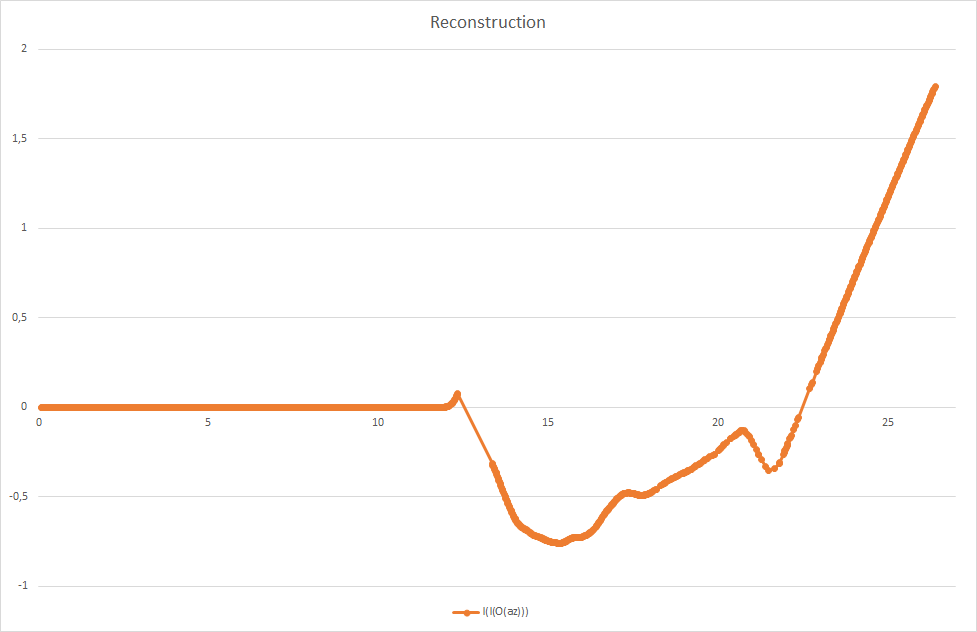
\includegraphics[width=15cm]{Pictures/Flight Reconst Offset.png}}
\fbox{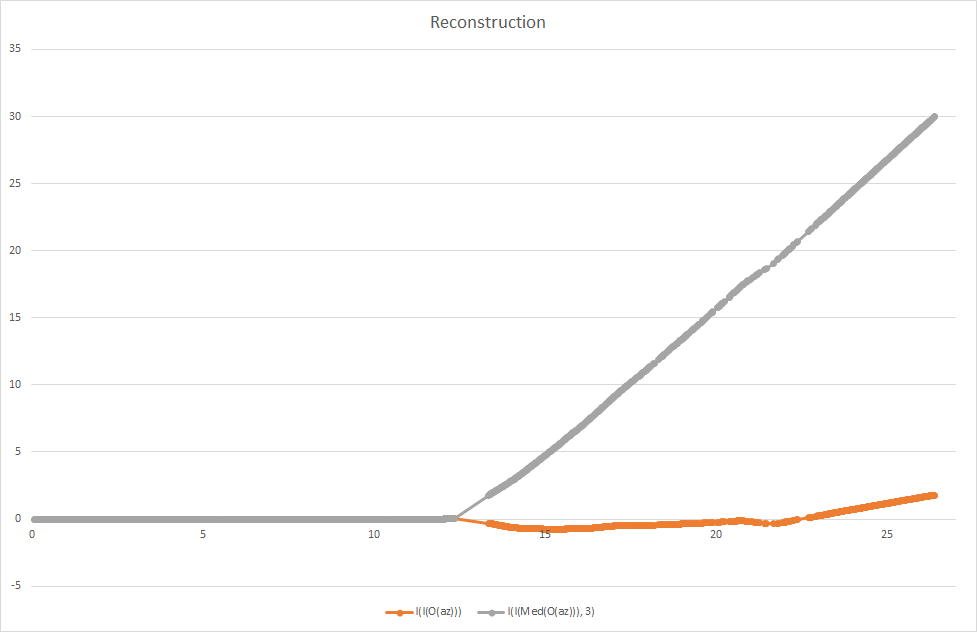
\includegraphics[width=7.31cm]{Pictures/Flight Reconst OffsetMedian.png}}
\fbox{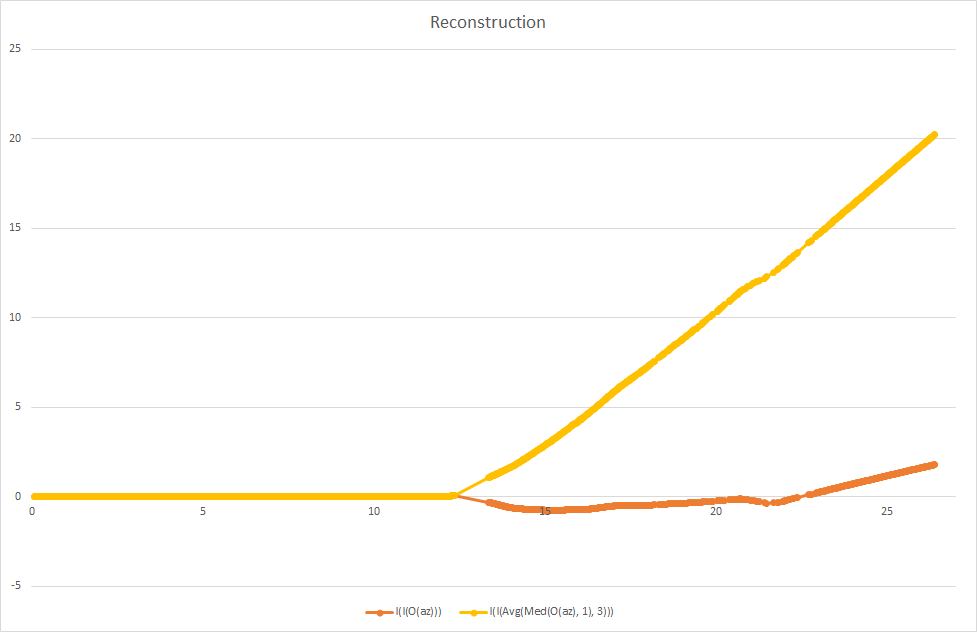
\includegraphics[width=7.31cm]{Pictures/Flight Reconst OffsetAverage.png}}
\caption{Testflug: Rekonstruktion der Flughöhe}
\label{fig:FlightHeightReconst}
\end{center}

\vspace{0.25cm}
Das Bild oben zeigt die doppelte Integration von Daten, von welchen eine konstante Abweichung subtrahiert wurde und in blau den gemessenen Höhenverlauf.\\
Für die Bilder unten wurde auf die abweichungskorrigierten Daten ein Median-Filter (links) und ein Mittelwert-Filter (rechts) angewandt.
\end{figure}






